\documentclass{article}
\usepackage[utf8]{inputenc}
\usepackage[spanish]{babel}
\usepackage{listings}
\usepackage{graphicx}
\graphicspath{ {images/} }
\usepackage{cite}

\begin{document}

\begin{titlepage}
    \begin{center}
        \vspace*{1cm}
            
        \Huge
        \textbf{Idealización proyecto final}
            
        \vspace{0.5cm}
        \LARGE
        Informática II
            
        \vspace{1.5cm}
            
        \textbf{Andrés Felipe Rendón Villada}
        \newline
        \textbf{Daniel Andrés Agudelo Garcia}
            
        \vfill
            
        \vspace{0.8cm}
            
        \Large
        Despartamento de Ingeniería Electrónica y Telecomunicaciones\\
        Universidad de Antioquia\\
        Medellín\\
        Marzo de 2021
            
    \end{center}
\end{titlepage}

\tableofcontents
\newpage
\section{Sección introductoria}\label{intro}
La programación cuenta con muchos ambitos en los cuales podremos crear programas para un objetivo en especifico, poniendo a prueba nuestros conocimientos como desarrolladores ; en esta ocasión realizare un juego usando el lenguaje de programacion c++ y el IDE Qt creator a continuacion podra encontrar una descripcion detallada de como fue el desarrollo del proyecto desde el inicio hasta tener listo el ejecutable del juego.

\section{Sección de contenido} \label{contenido}

\subsection{Descripción del juego}
El juego tendra por nombre "Darkness", un rpg donde nuestro personaje principal será un caballero el cuál en medio de su viaje llegará a Brawood donde se dará cuenta que un gran misterio envuelve a este lugar, el objetivo de nuestro personaje es lograr sobrevivir 3 dias, al final de cada noche el jugador debera enfrentar un boss, cuando el jugador llegue al amancer final dependiendo de la opcion escogida por el jugador podra obtener 1 de los 3 finales posibles, el juego contara con zonas diferentes, y variedad de items (espadas,Ecos de sangre para realizar mejoras de vida y/o arma,pistolas,latigos como ardaria secundaria) los cuales le serviran para superar jefes y mazmorras del juego.

\subsection{categoria del juego}
plataformas \\
accion aventura\\ 
edad: +8 años\\

\subsection{Historia del juego}
El jugador tomará el rol de un caballero, el cuál llega en medio de una noche al pueblo de Bradwood. Un pueblo el cuál es conocido por los atributos que poseen sus habitantes en la sangre los cuales fueron vendencidos por "La fiera deidad" que les otorgo la capacidad de curar diversas enfermedades usando su sangre , pero surgio una organizacion denominada "Bloodborne" la cual se encargaba de hacer el estudio de la sangre y experimentar la mezcla de hechiceria con la sangre esto provoco que su sangre se corrompiera causando que los habitantes se conviertan en bestias para evitar que la "darkblood" se esparciera el rey "blooded" conforma un escuadron de caballeros denominada "fieryrebels" cuya mision es impedir que la darkblood se esparza
y derrotar al creador de la "bloodborne" polux, el jugador tendra 3 dias para completar la mision.

\subsection{Personajes}

1. Personaje principal: Khorne\\
2. Rey de Brawood : "blooded"\\
3. Polux : Jefe de la bloodborne\\
4. jefe zona 1: por definir nombre\\
5, jefe zona 2: por definir nombre\\
6. jefe zona 3: por definir nombre\\

\subsection{Armas e Items}


\section{Inclusión de imágenes} \label{imagenes}

En la Figura (\ref{fig:Darkness}), se presenta el logo del juego Darkness contenido en la carpeta images.

\begin{figure}[h]
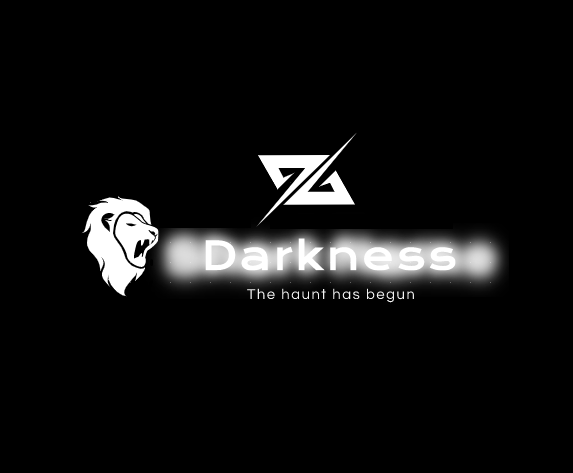
\includegraphics[width=4cm]{Darkness.PNG}
\centering
\caption{Logo de Darkness}
\label{fig:Darkness}
\end{figure}


\bibliographystyle{IEEEtran}
\bibliography{references}

\end{document}
